% Created by tikzDevice version 0.12.3.1 on 2022-10-23 12:15:00
% !TEX encoding = UTF-8 Unicode
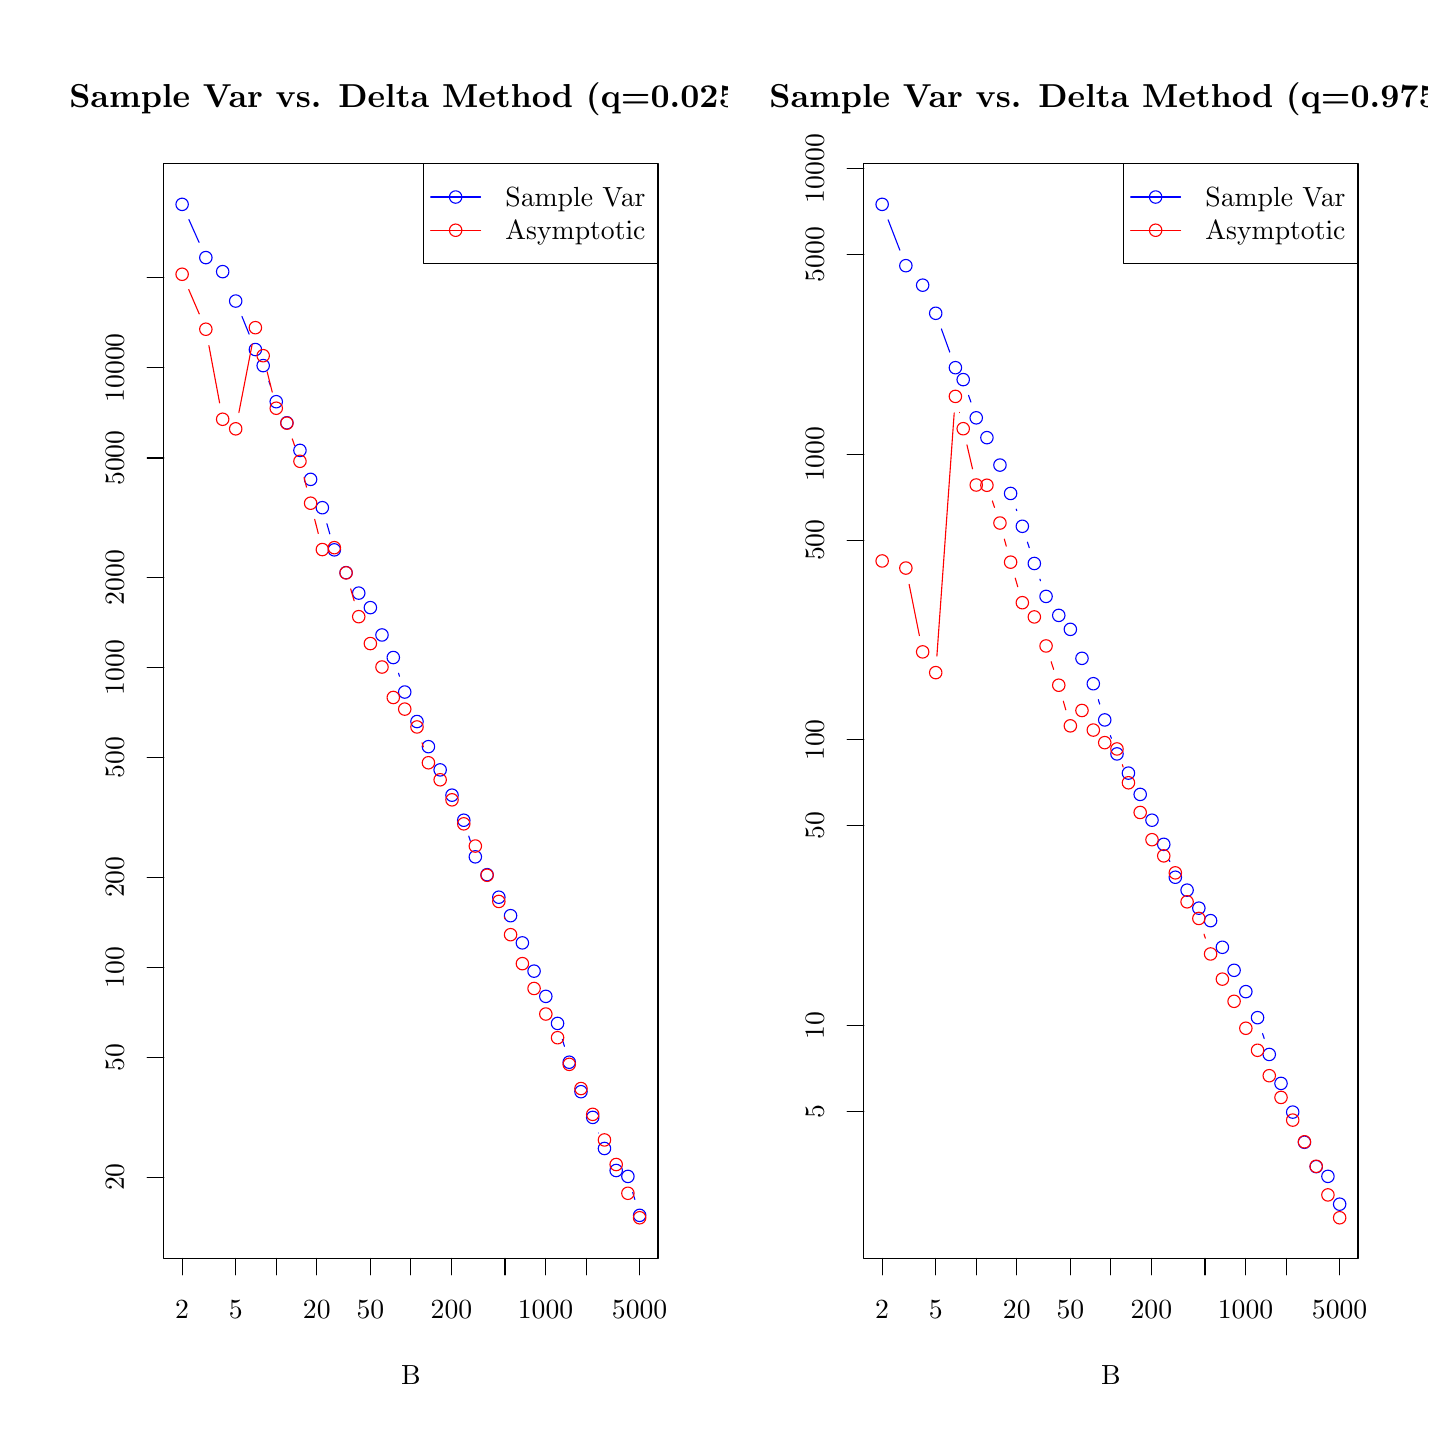
\begin{tikzpicture}[x=1pt,y=1pt]
\definecolor{fillColor}{RGB}{255,255,255}
\path[use as bounding box,fill=fillColor,fill opacity=0.00] (0,0) rectangle (505.89,505.89);
\begin{scope}
\path[clip] ( 49.20, 61.20) rectangle (227.75,456.69);
\definecolor{drawColor}{RGB}{0,0,255}

\path[draw=drawColor,line width= 0.4pt,line join=round,line cap=round] ( 58.25,436.56) -- ( 61.94,428.28);

\path[draw=drawColor,line width= 0.4pt,line join=round,line cap=round] ( 77.43,401.54) -- ( 80.03,395.13);

\path[draw=drawColor,line width= 0.4pt,line join=round,line cap=round] ( 87.15,378.12) -- ( 87.78,376.37);

\path[draw=drawColor,line width= 0.4pt,line join=round,line cap=round] (108.12,326.66) -- (109.17,322.96);

\path[draw=drawColor,line width= 0.4pt,line join=round,line cap=round] (134.00,272.60) -- (134.36,271.51);

\path[draw=drawColor,line width= 0.4pt,line join=round,line cap=round] (159.39,213.78) -- (159.95,211.99);

\path[draw=drawColor,line width= 0.4pt,line join=round,line cap=round] (193.20,140.33) -- (193.96,137.79);

\path[draw=drawColor,line width= 0.4pt,line join=round,line cap=round] (206.29,106.51) -- (206.30,106.50);

\path[draw=drawColor,line width= 0.4pt,line join=round,line cap=round] (218.62, 85.05) -- (219.40, 82.47);

\path[draw=drawColor,line width= 0.4pt,line join=round,line cap=round] ( 55.81,442.04) circle (  2.25);

\path[draw=drawColor,line width= 0.4pt,line join=round,line cap=round] ( 64.38,422.80) circle (  2.25);

\path[draw=drawColor,line width= 0.4pt,line join=round,line cap=round] ( 70.46,417.73) circle (  2.25);

\path[draw=drawColor,line width= 0.4pt,line join=round,line cap=round] ( 75.17,407.10) circle (  2.25);

\path[draw=drawColor,line width= 0.4pt,line join=round,line cap=round] ( 82.28,389.57) circle (  2.25);

\path[draw=drawColor,line width= 0.4pt,line join=round,line cap=round] ( 85.10,383.77) circle (  2.25);

\path[draw=drawColor,line width= 0.4pt,line join=round,line cap=round] ( 89.82,370.73) circle (  2.25);

\path[draw=drawColor,line width= 0.4pt,line join=round,line cap=round] ( 93.67,363.11) circle (  2.25);

\path[draw=drawColor,line width= 0.4pt,line join=round,line cap=round] ( 98.39,353.14) circle (  2.25);

\path[draw=drawColor,line width= 0.4pt,line join=round,line cap=round] (102.24,342.67) circle (  2.25);

\path[draw=drawColor,line width= 0.4pt,line join=round,line cap=round] (106.48,332.43) circle (  2.25);

\path[draw=drawColor,line width= 0.4pt,line join=round,line cap=round] (110.81,317.19) circle (  2.25);

\path[draw=drawColor,line width= 0.4pt,line join=round,line cap=round] (115.05,308.95) circle (  2.25);

\path[draw=drawColor,line width= 0.4pt,line join=round,line cap=round] (119.63,301.57) circle (  2.25);

\path[draw=drawColor,line width= 0.4pt,line join=round,line cap=round] (123.83,296.32) circle (  2.25);

\path[draw=drawColor,line width= 0.4pt,line join=round,line cap=round] (128.03,286.44) circle (  2.25);

\path[draw=drawColor,line width= 0.4pt,line join=round,line cap=round] (132.11,278.29) circle (  2.25);

\path[draw=drawColor,line width= 0.4pt,line join=round,line cap=round] (136.25,265.82) circle (  2.25);

\path[draw=drawColor,line width= 0.4pt,line join=round,line cap=round] (140.68,255.16) circle (  2.25);

\path[draw=drawColor,line width= 0.4pt,line join=round,line cap=round] (144.81,246.08) circle (  2.25);

\path[draw=drawColor,line width= 0.4pt,line join=round,line cap=round] (149.05,237.69) circle (  2.25);

\path[draw=drawColor,line width= 0.4pt,line join=round,line cap=round] (153.33,228.55) circle (  2.25);

\path[draw=drawColor,line width= 0.4pt,line join=round,line cap=round] (157.58,219.50) circle (  2.25);

\path[draw=drawColor,line width= 0.4pt,line join=round,line cap=round] (161.76,206.27) circle (  2.25);

\path[draw=drawColor,line width= 0.4pt,line join=round,line cap=round] (166.00,199.82) circle (  2.25);

\path[draw=drawColor,line width= 0.4pt,line join=round,line cap=round] (170.25,191.68) circle (  2.25);

\path[draw=drawColor,line width= 0.4pt,line join=round,line cap=round] (174.49,185.00) circle (  2.25);

\path[draw=drawColor,line width= 0.4pt,line join=round,line cap=round] (178.76,175.18) circle (  2.25);

\path[draw=drawColor,line width= 0.4pt,line join=round,line cap=round] (182.98,164.97) circle (  2.25);

\path[draw=drawColor,line width= 0.4pt,line join=round,line cap=round] (187.23,155.85) circle (  2.25);

\path[draw=drawColor,line width= 0.4pt,line join=round,line cap=round] (191.47,146.08) circle (  2.25);

\path[draw=drawColor,line width= 0.4pt,line join=round,line cap=round] (195.69,132.05) circle (  2.25);

\path[draw=drawColor,line width= 0.4pt,line join=round,line cap=round] (199.94,121.40) circle (  2.25);

\path[draw=drawColor,line width= 0.4pt,line join=round,line cap=round] (204.18,112.12) circle (  2.25);

\path[draw=drawColor,line width= 0.4pt,line join=round,line cap=round] (208.42,100.88) circle (  2.25);

\path[draw=drawColor,line width= 0.4pt,line join=round,line cap=round] (212.65, 92.93) circle (  2.25);

\path[draw=drawColor,line width= 0.4pt,line join=round,line cap=round] (216.89, 90.79) circle (  2.25);

\path[draw=drawColor,line width= 0.4pt,line join=round,line cap=round] (221.13, 76.72) circle (  2.25);
\end{scope}
\begin{scope}
\path[clip] (  0.00,  0.00) rectangle (505.89,505.89);
\definecolor{drawColor}{RGB}{0,0,0}

\path[draw=drawColor,line width= 0.4pt,line join=round,line cap=round] ( 55.81, 61.20) -- (221.13, 61.20);

\path[draw=drawColor,line width= 0.4pt,line join=round,line cap=round] ( 55.81, 61.20) -- ( 55.81, 55.20);

\path[draw=drawColor,line width= 0.4pt,line join=round,line cap=round] ( 75.17, 61.20) -- ( 75.17, 55.20);

\path[draw=drawColor,line width= 0.4pt,line join=round,line cap=round] ( 89.82, 61.20) -- ( 89.82, 55.20);

\path[draw=drawColor,line width= 0.4pt,line join=round,line cap=round] (104.47, 61.20) -- (104.47, 55.20);

\path[draw=drawColor,line width= 0.4pt,line join=round,line cap=round] (123.83, 61.20) -- (123.83, 55.20);

\path[draw=drawColor,line width= 0.4pt,line join=round,line cap=round] (138.47, 61.20) -- (138.47, 55.20);

\path[draw=drawColor,line width= 0.4pt,line join=round,line cap=round] (153.12, 61.20) -- (153.12, 55.20);

\path[draw=drawColor,line width= 0.4pt,line join=round,line cap=round] (172.48, 61.20) -- (172.48, 55.20);

\path[draw=drawColor,line width= 0.4pt,line join=round,line cap=round] (187.13, 61.20) -- (187.13, 55.20);

\path[draw=drawColor,line width= 0.4pt,line join=round,line cap=round] (201.77, 61.20) -- (201.77, 55.20);

\path[draw=drawColor,line width= 0.4pt,line join=round,line cap=round] (221.13, 61.20) -- (221.13, 55.20);

\node[text=drawColor,anchor=base,inner sep=0pt, outer sep=0pt, scale=  1.00] at ( 55.81, 39.60) {2};

\node[text=drawColor,anchor=base,inner sep=0pt, outer sep=0pt, scale=  1.00] at ( 75.17, 39.60) {5};

\node[text=drawColor,anchor=base,inner sep=0pt, outer sep=0pt, scale=  1.00] at (104.47, 39.60) {20};

\node[text=drawColor,anchor=base,inner sep=0pt, outer sep=0pt, scale=  1.00] at (123.83, 39.60) {50};

\node[text=drawColor,anchor=base,inner sep=0pt, outer sep=0pt, scale=  1.00] at (153.12, 39.60) {200};

\node[text=drawColor,anchor=base,inner sep=0pt, outer sep=0pt, scale=  1.00] at (187.13, 39.60) {1000};

\node[text=drawColor,anchor=base,inner sep=0pt, outer sep=0pt, scale=  1.00] at (221.13, 39.60) {5000};

\path[draw=drawColor,line width= 0.4pt,line join=round,line cap=round] ( 49.20, 90.55) -- ( 49.20,415.62);

\path[draw=drawColor,line width= 0.4pt,line join=round,line cap=round] ( 49.20, 90.55) -- ( 43.20, 90.55);

\path[draw=drawColor,line width= 0.4pt,line join=round,line cap=round] ( 49.20,133.67) -- ( 43.20,133.67);

\path[draw=drawColor,line width= 0.4pt,line join=round,line cap=round] ( 49.20,166.29) -- ( 43.20,166.29);

\path[draw=drawColor,line width= 0.4pt,line join=round,line cap=round] ( 49.20,198.91) -- ( 43.20,198.91);

\path[draw=drawColor,line width= 0.4pt,line join=round,line cap=round] ( 49.20,242.03) -- ( 43.20,242.03);

\path[draw=drawColor,line width= 0.4pt,line join=round,line cap=round] ( 49.20,274.64) -- ( 43.20,274.64);

\path[draw=drawColor,line width= 0.4pt,line join=round,line cap=round] ( 49.20,307.26) -- ( 43.20,307.26);

\path[draw=drawColor,line width= 0.4pt,line join=round,line cap=round] ( 49.20,350.38) -- ( 43.20,350.38);

\path[draw=drawColor,line width= 0.4pt,line join=round,line cap=round] ( 49.20,383.00) -- ( 43.20,383.00);

\path[draw=drawColor,line width= 0.4pt,line join=round,line cap=round] ( 49.20,415.62) -- ( 43.20,415.62);

\node[text=drawColor,rotate= 90.00,anchor=base,inner sep=0pt, outer sep=0pt, scale=  1.00] at ( 34.80, 90.55) {20};

\node[text=drawColor,rotate= 90.00,anchor=base,inner sep=0pt, outer sep=0pt, scale=  1.00] at ( 34.80,133.67) {50};

\node[text=drawColor,rotate= 90.00,anchor=base,inner sep=0pt, outer sep=0pt, scale=  1.00] at ( 34.80,166.29) {100};

\node[text=drawColor,rotate= 90.00,anchor=base,inner sep=0pt, outer sep=0pt, scale=  1.00] at ( 34.80,198.91) {200};

\node[text=drawColor,rotate= 90.00,anchor=base,inner sep=0pt, outer sep=0pt, scale=  1.00] at ( 34.80,242.03) {500};

\node[text=drawColor,rotate= 90.00,anchor=base,inner sep=0pt, outer sep=0pt, scale=  1.00] at ( 34.80,274.64) {1000};

\node[text=drawColor,rotate= 90.00,anchor=base,inner sep=0pt, outer sep=0pt, scale=  1.00] at ( 34.80,307.26) {2000};

\node[text=drawColor,rotate= 90.00,anchor=base,inner sep=0pt, outer sep=0pt, scale=  1.00] at ( 34.80,350.38) {5000};

\node[text=drawColor,rotate= 90.00,anchor=base,inner sep=0pt, outer sep=0pt, scale=  1.00] at ( 34.80,383.00) {10000};

\path[draw=drawColor,line width= 0.4pt,line join=round,line cap=round] ( 49.20, 61.20) --
	(227.75, 61.20) --
	(227.75,456.69) --
	( 49.20,456.69) --
	cycle;
\end{scope}
\begin{scope}
\path[clip] (  0.00,  0.00) rectangle (252.94,505.89);
\definecolor{drawColor}{RGB}{0,0,0}

\node[text=drawColor,anchor=base,inner sep=0pt, outer sep=0pt, scale=  1.20] at (138.47,477.15) {\bfseries Sample Var vs. Delta Method (q=0.025)};

\node[text=drawColor,anchor=base,inner sep=0pt, outer sep=0pt, scale=  1.00] at (138.47, 15.60) {B};
\end{scope}
\begin{scope}
\path[clip] ( 49.20, 61.20) rectangle (227.75,456.69);
\definecolor{drawColor}{RGB}{255,0,0}

\path[draw=drawColor,line width= 0.4pt,line join=round,line cap=round] ( 58.19,411.27) -- ( 62.00,402.43);

\path[draw=drawColor,line width= 0.4pt,line join=round,line cap=round] ( 65.48,391.02) -- ( 69.36,370.29);

\path[draw=drawColor,line width= 0.4pt,line join=round,line cap=round] ( 76.32,366.82) -- ( 81.14,391.59);

\path[draw=drawColor,line width= 0.4pt,line join=round,line cap=round] ( 86.55,381.53) -- ( 88.37,374.19);

\path[draw=drawColor,line width= 0.4pt,line join=round,line cap=round] ( 95.61,357.31) -- ( 96.45,354.87);

\path[draw=drawColor,line width= 0.4pt,line join=round,line cap=round] ( 99.87,343.38) -- (100.76,339.86);

\path[draw=drawColor,line width= 0.4pt,line join=round,line cap=round] (103.71,328.23) -- (105.01,323.11);

\path[draw=drawColor,line width= 0.4pt,line join=round,line cap=round] (116.72,303.11) -- (117.96,298.81);

\path[draw=drawColor,line width= 0.4pt,line join=round,line cap=round] (142.50,247.48) -- (142.99,245.97);

\path[draw=drawColor,line width= 0.4pt,line join=round,line cap=round] (172.25,184.49) -- (172.50,183.80);

\path[draw=drawColor,line width= 0.4pt,line join=round,line cap=round] ( 55.81,416.78) circle (  2.25);

\path[draw=drawColor,line width= 0.4pt,line join=round,line cap=round] ( 64.38,396.92) circle (  2.25);

\path[draw=drawColor,line width= 0.4pt,line join=round,line cap=round] ( 70.46,364.39) circle (  2.25);

\path[draw=drawColor,line width= 0.4pt,line join=round,line cap=round] ( 75.17,360.93) circle (  2.25);

\path[draw=drawColor,line width= 0.4pt,line join=round,line cap=round] ( 82.28,397.48) circle (  2.25);

\path[draw=drawColor,line width= 0.4pt,line join=round,line cap=round] ( 85.10,387.35) circle (  2.25);

\path[draw=drawColor,line width= 0.4pt,line join=round,line cap=round] ( 89.82,368.37) circle (  2.25);

\path[draw=drawColor,line width= 0.4pt,line join=round,line cap=round] ( 93.67,362.98) circle (  2.25);

\path[draw=drawColor,line width= 0.4pt,line join=round,line cap=round] ( 98.39,349.20) circle (  2.25);

\path[draw=drawColor,line width= 0.4pt,line join=round,line cap=round] (102.24,334.05) circle (  2.25);

\path[draw=drawColor,line width= 0.4pt,line join=round,line cap=round] (106.48,317.30) circle (  2.25);

\path[draw=drawColor,line width= 0.4pt,line join=round,line cap=round] (110.81,317.98) circle (  2.25);

\path[draw=drawColor,line width= 0.4pt,line join=round,line cap=round] (115.05,308.88) circle (  2.25);

\path[draw=drawColor,line width= 0.4pt,line join=round,line cap=round] (119.63,293.05) circle (  2.25);

\path[draw=drawColor,line width= 0.4pt,line join=round,line cap=round] (123.83,283.33) circle (  2.25);

\path[draw=drawColor,line width= 0.4pt,line join=round,line cap=round] (128.03,274.86) circle (  2.25);

\path[draw=drawColor,line width= 0.4pt,line join=round,line cap=round] (132.11,263.85) circle (  2.25);

\path[draw=drawColor,line width= 0.4pt,line join=round,line cap=round] (136.25,259.65) circle (  2.25);

\path[draw=drawColor,line width= 0.4pt,line join=round,line cap=round] (140.68,253.20) circle (  2.25);

\path[draw=drawColor,line width= 0.4pt,line join=round,line cap=round] (144.81,240.26) circle (  2.25);

\path[draw=drawColor,line width= 0.4pt,line join=round,line cap=round] (149.05,234.11) circle (  2.25);

\path[draw=drawColor,line width= 0.4pt,line join=round,line cap=round] (153.33,226.87) circle (  2.25);

\path[draw=drawColor,line width= 0.4pt,line join=round,line cap=round] (157.58,218.19) circle (  2.25);

\path[draw=drawColor,line width= 0.4pt,line join=round,line cap=round] (161.76,210.17) circle (  2.25);

\path[draw=drawColor,line width= 0.4pt,line join=round,line cap=round] (166.00,199.61) circle (  2.25);

\path[draw=drawColor,line width= 0.4pt,line join=round,line cap=round] (170.25,190.15) circle (  2.25);

\path[draw=drawColor,line width= 0.4pt,line join=round,line cap=round] (174.49,178.14) circle (  2.25);

\path[draw=drawColor,line width= 0.4pt,line join=round,line cap=round] (178.76,167.67) circle (  2.25);

\path[draw=drawColor,line width= 0.4pt,line join=round,line cap=round] (182.98,158.70) circle (  2.25);

\path[draw=drawColor,line width= 0.4pt,line join=round,line cap=round] (187.23,149.47) circle (  2.25);

\path[draw=drawColor,line width= 0.4pt,line join=round,line cap=round] (191.47,140.91) circle (  2.25);

\path[draw=drawColor,line width= 0.4pt,line join=round,line cap=round] (195.69,131.29) circle (  2.25);

\path[draw=drawColor,line width= 0.4pt,line join=round,line cap=round] (199.94,122.54) circle (  2.25);

\path[draw=drawColor,line width= 0.4pt,line join=round,line cap=round] (204.18,113.22) circle (  2.25);

\path[draw=drawColor,line width= 0.4pt,line join=round,line cap=round] (208.42,103.97) circle (  2.25);

\path[draw=drawColor,line width= 0.4pt,line join=round,line cap=round] (212.65, 95.09) circle (  2.25);

\path[draw=drawColor,line width= 0.4pt,line join=round,line cap=round] (216.89, 84.70) circle (  2.25);

\path[draw=drawColor,line width= 0.4pt,line join=round,line cap=round] (221.13, 75.85) circle (  2.25);
\definecolor{drawColor}{RGB}{0,0,0}

\path[draw=drawColor,line width= 0.4pt,line join=round,line cap=round] (142.95,456.69) rectangle (227.75,420.69);
\definecolor{drawColor}{RGB}{0,0,255}

\path[draw=drawColor,line width= 0.4pt,line join=round,line cap=round] (145.65,444.69) -- (163.65,444.69);
\definecolor{drawColor}{RGB}{255,0,0}

\path[draw=drawColor,line width= 0.4pt,line join=round,line cap=round] (145.65,432.69) -- (163.65,432.69);
\definecolor{drawColor}{RGB}{0,0,255}

\path[draw=drawColor,line width= 0.4pt,line join=round,line cap=round] (154.65,444.69) circle (  2.25);
\definecolor{drawColor}{RGB}{255,0,0}

\path[draw=drawColor,line width= 0.4pt,line join=round,line cap=round] (154.65,432.69) circle (  2.25);
\definecolor{drawColor}{RGB}{0,0,0}

\node[text=drawColor,anchor=base west,inner sep=0pt, outer sep=0pt, scale=  1.00] at (172.65,441.25) {Sample Var};

\node[text=drawColor,anchor=base west,inner sep=0pt, outer sep=0pt, scale=  1.00] at (172.65,429.25) {Asymptotic};
\end{scope}
\begin{scope}
\path[clip] (302.14, 61.20) rectangle (480.69,456.69);
\definecolor{drawColor}{RGB}{0,0,255}

\path[draw=drawColor,line width= 0.4pt,line join=round,line cap=round] (310.92,436.45) -- (315.16,425.47);

\path[draw=drawColor,line width= 0.4pt,line join=round,line cap=round] (330.16,397.04) -- (333.19,388.66);

\path[draw=drawColor,line width= 0.4pt,line join=round,line cap=round] (339.99,373.03) -- (340.83,370.58);

\path[draw=drawColor,line width= 0.4pt,line join=round,line cap=round] (357.20,331.93) -- (357.41,331.36);

\path[draw=drawColor,line width= 0.4pt,line join=round,line cap=round] (361.26,320.00) -- (361.91,317.98);

\path[draw=drawColor,line width= 0.4pt,line join=round,line cap=round] (365.77,306.62) -- (365.98,306.02);

\path[draw=drawColor,line width= 0.4pt,line join=round,line cap=round] (386.86,263.10) -- (387.38,261.46);

\path[draw=drawColor,line width= 0.4pt,line join=round,line cap=round] (391.23,250.09) -- (391.59,249.11);

\path[draw=drawColor,line width= 0.4pt,line join=round,line cap=round] (412.51,205.13) -- (412.71,204.56);

\path[draw=drawColor,line width= 0.4pt,line join=round,line cap=round] (446.23,142.43) -- (446.82,140.58);

\path[draw=drawColor,line width= 0.4pt,line join=round,line cap=round] (308.76,442.04) circle (  2.25);

\path[draw=drawColor,line width= 0.4pt,line join=round,line cap=round] (317.33,419.88) circle (  2.25);

\path[draw=drawColor,line width= 0.4pt,line join=round,line cap=round] (323.40,412.84) circle (  2.25);

\path[draw=drawColor,line width= 0.4pt,line join=round,line cap=round] (328.12,402.68) circle (  2.25);

\path[draw=drawColor,line width= 0.4pt,line join=round,line cap=round] (335.23,383.02) circle (  2.25);

\path[draw=drawColor,line width= 0.4pt,line join=round,line cap=round] (338.05,378.71) circle (  2.25);

\path[draw=drawColor,line width= 0.4pt,line join=round,line cap=round] (342.76,364.90) circle (  2.25);

\path[draw=drawColor,line width= 0.4pt,line join=round,line cap=round] (346.62,357.74) circle (  2.25);

\path[draw=drawColor,line width= 0.4pt,line join=round,line cap=round] (351.33,347.83) circle (  2.25);

\path[draw=drawColor,line width= 0.4pt,line join=round,line cap=round] (355.18,337.58) circle (  2.25);

\path[draw=drawColor,line width= 0.4pt,line join=round,line cap=round] (359.42,325.71) circle (  2.25);

\path[draw=drawColor,line width= 0.4pt,line join=round,line cap=round] (363.75,312.27) circle (  2.25);

\path[draw=drawColor,line width= 0.4pt,line join=round,line cap=round] (367.99,300.37) circle (  2.25);

\path[draw=drawColor,line width= 0.4pt,line join=round,line cap=round] (372.58,293.52) circle (  2.25);

\path[draw=drawColor,line width= 0.4pt,line join=round,line cap=round] (376.77,288.47) circle (  2.25);

\path[draw=drawColor,line width= 0.4pt,line join=round,line cap=round] (380.97,278.00) circle (  2.25);

\path[draw=drawColor,line width= 0.4pt,line join=round,line cap=round] (385.06,268.82) circle (  2.25);

\path[draw=drawColor,line width= 0.4pt,line join=round,line cap=round] (389.19,255.74) circle (  2.25);

\path[draw=drawColor,line width= 0.4pt,line join=round,line cap=round] (393.62,243.46) circle (  2.25);

\path[draw=drawColor,line width= 0.4pt,line join=round,line cap=round] (397.76,236.52) circle (  2.25);

\path[draw=drawColor,line width= 0.4pt,line join=round,line cap=round] (402.00,228.83) circle (  2.25);

\path[draw=drawColor,line width= 0.4pt,line join=round,line cap=round] (406.27,219.51) circle (  2.25);

\path[draw=drawColor,line width= 0.4pt,line join=round,line cap=round] (410.52,210.79) circle (  2.25);

\path[draw=drawColor,line width= 0.4pt,line join=round,line cap=round] (414.70,198.90) circle (  2.25);

\path[draw=drawColor,line width= 0.4pt,line join=round,line cap=round] (418.95,194.23) circle (  2.25);

\path[draw=drawColor,line width= 0.4pt,line join=round,line cap=round] (423.20,187.73) circle (  2.25);

\path[draw=drawColor,line width= 0.4pt,line join=round,line cap=round] (427.44,183.21) circle (  2.25);

\path[draw=drawColor,line width= 0.4pt,line join=round,line cap=round] (431.70,173.59) circle (  2.25);

\path[draw=drawColor,line width= 0.4pt,line join=round,line cap=round] (435.93,165.27) circle (  2.25);

\path[draw=drawColor,line width= 0.4pt,line join=round,line cap=round] (440.18,157.56) circle (  2.25);

\path[draw=drawColor,line width= 0.4pt,line join=round,line cap=round] (444.41,148.15) circle (  2.25);

\path[draw=drawColor,line width= 0.4pt,line join=round,line cap=round] (448.64,134.86) circle (  2.25);

\path[draw=drawColor,line width= 0.4pt,line join=round,line cap=round] (452.89,124.40) circle (  2.25);

\path[draw=drawColor,line width= 0.4pt,line join=round,line cap=round] (457.12,114.03) circle (  2.25);

\path[draw=drawColor,line width= 0.4pt,line join=round,line cap=round] (461.36,103.13) circle (  2.25);

\path[draw=drawColor,line width= 0.4pt,line join=round,line cap=round] (465.60, 94.32) circle (  2.25);

\path[draw=drawColor,line width= 0.4pt,line join=round,line cap=round] (469.84, 90.81) circle (  2.25);

\path[draw=drawColor,line width= 0.4pt,line join=round,line cap=round] (474.08, 80.76) circle (  2.25);
\end{scope}
\begin{scope}
\path[clip] (  0.00,  0.00) rectangle (505.89,505.89);
\definecolor{drawColor}{RGB}{0,0,0}

\path[draw=drawColor,line width= 0.4pt,line join=round,line cap=round] (308.76, 61.20) -- (474.08, 61.20);

\path[draw=drawColor,line width= 0.4pt,line join=round,line cap=round] (308.76, 61.20) -- (308.76, 55.20);

\path[draw=drawColor,line width= 0.4pt,line join=round,line cap=round] (328.12, 61.20) -- (328.12, 55.20);

\path[draw=drawColor,line width= 0.4pt,line join=round,line cap=round] (342.76, 61.20) -- (342.76, 55.20);

\path[draw=drawColor,line width= 0.4pt,line join=round,line cap=round] (357.41, 61.20) -- (357.41, 55.20);

\path[draw=drawColor,line width= 0.4pt,line join=round,line cap=round] (376.77, 61.20) -- (376.77, 55.20);

\path[draw=drawColor,line width= 0.4pt,line join=round,line cap=round] (391.42, 61.20) -- (391.42, 55.20);

\path[draw=drawColor,line width= 0.4pt,line join=round,line cap=round] (406.06, 61.20) -- (406.06, 55.20);

\path[draw=drawColor,line width= 0.4pt,line join=round,line cap=round] (425.42, 61.20) -- (425.42, 55.20);

\path[draw=drawColor,line width= 0.4pt,line join=round,line cap=round] (440.07, 61.20) -- (440.07, 55.20);

\path[draw=drawColor,line width= 0.4pt,line join=round,line cap=round] (454.72, 61.20) -- (454.72, 55.20);

\path[draw=drawColor,line width= 0.4pt,line join=round,line cap=round] (474.08, 61.20) -- (474.08, 55.20);

\node[text=drawColor,anchor=base,inner sep=0pt, outer sep=0pt, scale=  1.00] at (308.76, 39.60) {2};

\node[text=drawColor,anchor=base,inner sep=0pt, outer sep=0pt, scale=  1.00] at (328.12, 39.60) {5};

\node[text=drawColor,anchor=base,inner sep=0pt, outer sep=0pt, scale=  1.00] at (357.41, 39.60) {20};

\node[text=drawColor,anchor=base,inner sep=0pt, outer sep=0pt, scale=  1.00] at (376.77, 39.60) {50};

\node[text=drawColor,anchor=base,inner sep=0pt, outer sep=0pt, scale=  1.00] at (406.06, 39.60) {200};

\node[text=drawColor,anchor=base,inner sep=0pt, outer sep=0pt, scale=  1.00] at (440.07, 39.60) {1000};

\node[text=drawColor,anchor=base,inner sep=0pt, outer sep=0pt, scale=  1.00] at (474.08, 39.60) {5000};

\path[draw=drawColor,line width= 0.4pt,line join=round,line cap=round] (302.14,114.19) -- (302.14,455.01);

\path[draw=drawColor,line width= 0.4pt,line join=round,line cap=round] (302.14,114.19) -- (296.14,114.19);

\path[draw=drawColor,line width= 0.4pt,line join=round,line cap=round] (302.14,145.27) -- (296.14,145.27);

\path[draw=drawColor,line width= 0.4pt,line join=round,line cap=round] (302.14,217.44) -- (296.14,217.44);

\path[draw=drawColor,line width= 0.4pt,line join=round,line cap=round] (302.14,248.52) -- (296.14,248.52);

\path[draw=drawColor,line width= 0.4pt,line join=round,line cap=round] (302.14,320.69) -- (296.14,320.69);

\path[draw=drawColor,line width= 0.4pt,line join=round,line cap=round] (302.14,351.77) -- (296.14,351.77);

\path[draw=drawColor,line width= 0.4pt,line join=round,line cap=round] (302.14,423.93) -- (296.14,423.93);

\path[draw=drawColor,line width= 0.4pt,line join=round,line cap=round] (302.14,455.01) -- (296.14,455.01);

\node[text=drawColor,rotate= 90.00,anchor=base,inner sep=0pt, outer sep=0pt, scale=  1.00] at (287.75,114.19) {5};

\node[text=drawColor,rotate= 90.00,anchor=base,inner sep=0pt, outer sep=0pt, scale=  1.00] at (287.75,145.27) {10};

\node[text=drawColor,rotate= 90.00,anchor=base,inner sep=0pt, outer sep=0pt, scale=  1.00] at (287.75,217.44) {50};

\node[text=drawColor,rotate= 90.00,anchor=base,inner sep=0pt, outer sep=0pt, scale=  1.00] at (287.75,248.52) {100};

\node[text=drawColor,rotate= 90.00,anchor=base,inner sep=0pt, outer sep=0pt, scale=  1.00] at (287.75,320.69) {500};

\node[text=drawColor,rotate= 90.00,anchor=base,inner sep=0pt, outer sep=0pt, scale=  1.00] at (287.75,351.77) {1000};

\node[text=drawColor,rotate= 90.00,anchor=base,inner sep=0pt, outer sep=0pt, scale=  1.00] at (287.75,423.93) {5000};

\node[text=drawColor,rotate= 90.00,anchor=base,inner sep=0pt, outer sep=0pt, scale=  1.00] at (287.75,455.01) {10000};

\path[draw=drawColor,line width= 0.4pt,line join=round,line cap=round] (302.14, 61.20) --
	(480.69, 61.20) --
	(480.69,456.69) --
	(302.14,456.69) --
	cycle;
\end{scope}
\begin{scope}
\path[clip] (252.94,  0.00) rectangle (505.89,505.89);
\definecolor{drawColor}{RGB}{0,0,0}

\node[text=drawColor,anchor=base,inner sep=0pt, outer sep=0pt, scale=  1.20] at (391.42,477.15) {\bfseries Sample Var vs. Delta Method (q=0.975)};

\node[text=drawColor,anchor=base,inner sep=0pt, outer sep=0pt, scale=  1.00] at (391.42, 15.60) {B};
\end{scope}
\begin{scope}
\path[clip] (302.14, 61.20) rectangle (480.69,456.69);
\definecolor{drawColor}{RGB}{255,0,0}

\path[draw=drawColor,line width= 0.4pt,line join=round,line cap=round] (318.51,304.73) -- (322.22,286.22);

\path[draw=drawColor,line width= 0.4pt,line join=round,line cap=round] (328.54,278.81) -- (334.80,366.67);

\path[draw=drawColor,line width= 0.4pt,line join=round,line cap=round] (336.64,366.82) -- (336.64,366.80);

\path[draw=drawColor,line width= 0.4pt,line join=round,line cap=round] (339.40,355.13) -- (341.41,346.48);

\path[draw=drawColor,line width= 0.4pt,line join=round,line cap=round] (348.58,334.87) -- (349.37,332.56);

\path[draw=drawColor,line width= 0.4pt,line join=round,line cap=round] (352.91,321.10) -- (353.61,318.54);

\path[draw=drawColor,line width= 0.4pt,line join=round,line cap=round] (356.85,306.99) -- (357.76,303.86);

\path[draw=drawColor,line width= 0.4pt,line join=round,line cap=round] (369.84,276.76) -- (370.73,273.99);

\path[draw=drawColor,line width= 0.4pt,line join=round,line cap=round] (374.23,262.51) -- (375.12,259.37);

\path[draw=drawColor,line width= 0.4pt,line join=round,line cap=round] (395.55,239.56) -- (395.83,238.71);

\path[draw=drawColor,line width= 0.4pt,line join=round,line cap=round] (425.08,178.31) -- (425.56,176.87);

\path[draw=drawColor,line width= 0.4pt,line join=round,line cap=round] (308.76,313.18) circle (  2.25);

\path[draw=drawColor,line width= 0.4pt,line join=round,line cap=round] (317.33,310.62) circle (  2.25);

\path[draw=drawColor,line width= 0.4pt,line join=round,line cap=round] (323.40,280.33) circle (  2.25);

\path[draw=drawColor,line width= 0.4pt,line join=round,line cap=round] (328.12,272.83) circle (  2.25);

\path[draw=drawColor,line width= 0.4pt,line join=round,line cap=round] (335.23,372.65) circle (  2.25);

\path[draw=drawColor,line width= 0.4pt,line join=round,line cap=round] (338.05,360.97) circle (  2.25);

\path[draw=drawColor,line width= 0.4pt,line join=round,line cap=round] (342.76,340.63) circle (  2.25);

\path[draw=drawColor,line width= 0.4pt,line join=round,line cap=round] (346.62,340.54) circle (  2.25);

\path[draw=drawColor,line width= 0.4pt,line join=round,line cap=round] (351.33,326.89) circle (  2.25);

\path[draw=drawColor,line width= 0.4pt,line join=round,line cap=round] (355.18,312.75) circle (  2.25);

\path[draw=drawColor,line width= 0.4pt,line join=round,line cap=round] (359.42,298.10) circle (  2.25);

\path[draw=drawColor,line width= 0.4pt,line join=round,line cap=round] (363.75,292.96) circle (  2.25);

\path[draw=drawColor,line width= 0.4pt,line join=round,line cap=round] (367.99,282.47) circle (  2.25);

\path[draw=drawColor,line width= 0.4pt,line join=round,line cap=round] (372.58,268.28) circle (  2.25);

\path[draw=drawColor,line width= 0.4pt,line join=round,line cap=round] (376.77,253.60) circle (  2.25);

\path[draw=drawColor,line width= 0.4pt,line join=round,line cap=round] (380.97,259.15) circle (  2.25);

\path[draw=drawColor,line width= 0.4pt,line join=round,line cap=round] (385.06,252.08) circle (  2.25);

\path[draw=drawColor,line width= 0.4pt,line join=round,line cap=round] (389.19,247.53) circle (  2.25);

\path[draw=drawColor,line width= 0.4pt,line join=round,line cap=round] (393.62,245.25) circle (  2.25);

\path[draw=drawColor,line width= 0.4pt,line join=round,line cap=round] (397.76,233.03) circle (  2.25);

\path[draw=drawColor,line width= 0.4pt,line join=round,line cap=round] (402.00,222.30) circle (  2.25);

\path[draw=drawColor,line width= 0.4pt,line join=round,line cap=round] (406.27,212.46) circle (  2.25);

\path[draw=drawColor,line width= 0.4pt,line join=round,line cap=round] (410.52,206.62) circle (  2.25);

\path[draw=drawColor,line width= 0.4pt,line join=round,line cap=round] (414.70,200.48) circle (  2.25);

\path[draw=drawColor,line width= 0.4pt,line join=round,line cap=round] (418.95,190.02) circle (  2.25);

\path[draw=drawColor,line width= 0.4pt,line join=round,line cap=round] (423.20,184.01) circle (  2.25);

\path[draw=drawColor,line width= 0.4pt,line join=round,line cap=round] (427.44,171.17) circle (  2.25);

\path[draw=drawColor,line width= 0.4pt,line join=round,line cap=round] (431.70,162.08) circle (  2.25);

\path[draw=drawColor,line width= 0.4pt,line join=round,line cap=round] (435.93,154.06) circle (  2.25);

\path[draw=drawColor,line width= 0.4pt,line join=round,line cap=round] (440.18,144.33) circle (  2.25);

\path[draw=drawColor,line width= 0.4pt,line join=round,line cap=round] (444.41,136.37) circle (  2.25);

\path[draw=drawColor,line width= 0.4pt,line join=round,line cap=round] (448.64,127.18) circle (  2.25);

\path[draw=drawColor,line width= 0.4pt,line join=round,line cap=round] (452.89,119.33) circle (  2.25);

\path[draw=drawColor,line width= 0.4pt,line join=round,line cap=round] (457.12,111.14) circle (  2.25);

\path[draw=drawColor,line width= 0.4pt,line join=round,line cap=round] (461.36,103.30) circle (  2.25);

\path[draw=drawColor,line width= 0.4pt,line join=round,line cap=round] (465.60, 94.45) circle (  2.25);

\path[draw=drawColor,line width= 0.4pt,line join=round,line cap=round] (469.84, 84.11) circle (  2.25);

\path[draw=drawColor,line width= 0.4pt,line join=round,line cap=round] (474.08, 75.85) circle (  2.25);
\definecolor{drawColor}{RGB}{0,0,0}

\path[draw=drawColor,line width= 0.4pt,line join=round,line cap=round] (395.89,456.69) rectangle (480.69,420.69);
\definecolor{drawColor}{RGB}{0,0,255}

\path[draw=drawColor,line width= 0.4pt,line join=round,line cap=round] (398.59,444.69) -- (416.59,444.69);
\definecolor{drawColor}{RGB}{255,0,0}

\path[draw=drawColor,line width= 0.4pt,line join=round,line cap=round] (398.59,432.69) -- (416.59,432.69);
\definecolor{drawColor}{RGB}{0,0,255}

\path[draw=drawColor,line width= 0.4pt,line join=round,line cap=round] (407.59,444.69) circle (  2.25);
\definecolor{drawColor}{RGB}{255,0,0}

\path[draw=drawColor,line width= 0.4pt,line join=round,line cap=round] (407.59,432.69) circle (  2.25);
\definecolor{drawColor}{RGB}{0,0,0}

\node[text=drawColor,anchor=base west,inner sep=0pt, outer sep=0pt, scale=  1.00] at (425.59,441.25) {Sample Var};

\node[text=drawColor,anchor=base west,inner sep=0pt, outer sep=0pt, scale=  1.00] at (425.59,429.25) {Asymptotic};
\end{scope}
\end{tikzpicture}